% !TeX root = main.tex
\section{Results and Discussion}
\label{sec:findings}
This section presents the study's descriptive and inferential statistics results, followed by a discussion of the findings.

The results of descriptive statistics revealed that 9\% of the participants rated extraversion, 14\% rated neuroticism, 17\% rated openness to experience, 28\% rated agreeableness, and 32\% rated conscientiousness as their dominant personality traits. Table \ref{tab:correl} shows the pearson's correlations between the big-five personality traits. 

\begin{table}[h]
  \centering
  \caption{Correlations between the Big-Five Traits\label{tab:correl}}
  \vspace{-12pt}
  \begin{tabular}{p{3cm}rrrrr}
    \toprule
    Trait & N & E & O & A & C \\\midrule
    Neuroticism (N) & 1.00 & -0.35 & 0.00 & -0.09 & -0.48 \\
    Extraversion (E) & -0.35 & 1.00 & 0.17 & 0.05 &	0.22 \\
    Openness (O) & 0.00 & 0.17 & 1.00 &	0.15 & -0.07 \\
    Agreeableness (A) & -0.09 &	0.05 & 0.15 & 1.00 & 0.43 \\ 
    Conscientiousness (C) & -0.48 & 0.22 & -0.07 &	0.43 &	1.00  \\\bottomrule
  \end{tabular}\vspace{-8pt}
\end{table}

Additionally, utilizing the plagiarism scores obtained from MOSS for both assignments, students were categorized into plagiarism levels according to the criteria outlined by the University Grants Commission (UGC) \cite{UGCPlagiarism}, a statutory body overseeing higher education in India. The outcomes are detailed in table \ref{tab:levelsPlagiarism}.

\begin{table}[h]
  \centering
  \caption{Percentage of students (N=105) falling in each Levels of Plagiarism \label{tab:levelsPlagiarism}}
  \vspace{-12pt}
  \begin{tabular}{p{1cm}p{2cm}rr}
    \toprule
    Level & Similarity \% & Assignment 1 & Assignment 2 \\\midrule
    Level 0 & Less than 10\% & 44.76\% & 40.95\% \\
    Level 1 & 10\% to 40\% & 27.51\% & 40.00\%  \\
    Level 2 & 41\% to 60\% & 14.28\% & 7.61\% \\
    Level 3 & More than 60\% &13.33\% & 11.42\% \\ \bottomrule
  \end{tabular}\vspace{-8pt}
\end{table}

\subsection{RQ1: Influence of Big-Five traits on Plagiarism}

One of the linear multiple regression assumptions is that the independent variables must not exhibit high (>5) multicollinearity. The multicollinearity between the five personality traits was tested using the variance inflation factor (VIF) and shown in Table \ref{tab:VIF}. All the VIF values were less than 5, indicating that multiple linear regression can be performed. 

\begin{table}[h]
  \centering
  \caption{Big-Five traits and their VIF\label{tab:VIF}}
    \vspace{-12pt}
  \begin{tabular}{p{2cm}r}
    \toprule
    Trait & VIF Value \\\midrule
    Neuroticism & 1.46 \\
    Extraversion & 1.20 \\
    Openness & 1.10\\
    Agreeableness & 1.33 \\ 
    Conscientiousness & 1.70  \\\bottomrule
  \end{tabular}\vspace{-4pt}
\end{table}

Multiple linear regression analyses were conducted with the big-five personality traits serving as the independent variables and the plagiarism score as the dependent variable for both assignments. The ordinary least squares (OLS) method was employed for the analysis, and the outcomes are displayed in Table \ref{tab:assign1Regression} and Table \ref{tab:assign2Regression}.

\begin{table}[h]
  \centering
  \caption{Regression analysis on Assignment 1 with $R^2$=0.106\\\label{tab:assign1Regression}}
    \vspace{-12pt}
  \begin{tabular}{p{2.5cm}rrrr}
    \toprule
    Trait & Coef & Std Err & \textit{t} & \textit{p}\\\midrule
    Agreeableness & 0.3489 & 0.243 & 1.434 & 0.155 \\
    Openness & -0.3401 & 0.256 & -1.328 & 0.187 \\
    Neuroticism & -0.1314 & 0.197 & -0.666 & 0.507 \\
    Extraversion & 0.6078 & 0.216 & 2.809 & 0.006* \\
    Conscientiousness & -0.2667 & 0.239 & -1.114 & 0.026* \\\bottomrule
  \end{tabular}\vspace{-4pt}
\end{table}

\begin{table}[ht]
  \centering
  \caption{Regression analysis on Assignment 2 with $R^2$=0.128\\\label{tab:assign2Regression}}
    \vspace{-12pt}
  \begin{tabular}{p{2.5cm}rrrr}
    \toprule
    Trait & Coef & Std Err & \textit{t} & \textit{p}\\\midrule
    Agreeableness & 0.3291 & 0.211 & 1.561 & 0.122 \\
    Openness & -0.3750 & 0.222 & -1.691 & 0.094\\
    Neuroticism & -0.2919 & 0.171 & -1.708 &  0.091\\
    Extraversion & 0.4394 & 0.187 & 2.344 & 0.021*\\
    Conscientiousness & -0.5541 & 0.207 & -2.673 & 0.009*\\\bottomrule
  \end{tabular}\vspace{-8pt}
\end{table}

Based on the findings from both assignments, irrespective of the actual coefficient values, it is apparent that extraversion exhibits a positive association with plagiarism (\textit{p}<0.05), while conscientiousness demonstrates a negative association with plagiarism (\textit{p}<0.05). However, the other personality traits are not statistically significant (\textit{p} values greater than 0.05).

\vspace{4pt}
\begin{mdframed}
\textbf{\textit{RQ1 Answer:}} Extraversion and conscientiousness traits influence plagiarism, with extraversion positively associated and conscientiousness negatively associated. The other three traits do not show a significant influence on plagiarism. 
\end{mdframed}
\vspace{4pt}

Some of these observations align with those reported in the literature, as illustrated in Table \ref{tab:litSUmmary}. For example, the lack of significance for openness to experience and neuroticism, as well as the negative association of conscientiousness with plagiarism, are consistent with the findings of Wilks et al. \cite{Wilks2016-WILPTA-3} and Giluk et al. \cite{Giluk2015BigFP}. However, in our study, extraversion demonstrates a positive association with plagiarism, consistent with the findings of Bhutto et al. \cite{Bhutto2019ACS} as shown in Fig\ref{fig:personalityAndPlagiarism}.

\begin{figure}[ht]
  \centering\vspace{-8pt}
  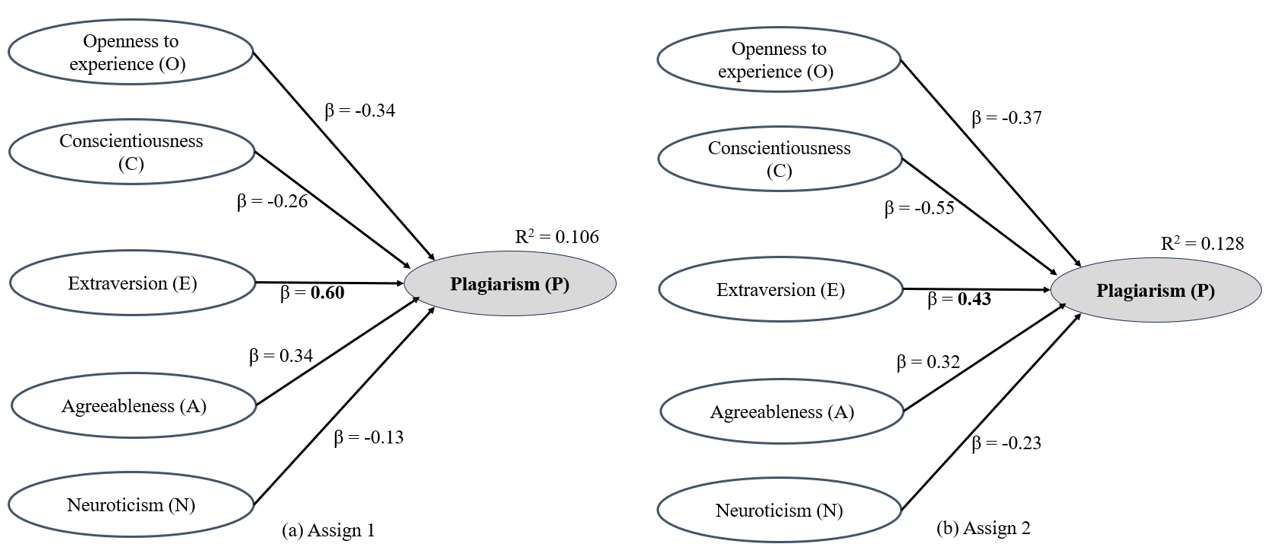
\includegraphics[width=\columnwidth]{1.png}
  \caption{The relationship between the big five traits in (a) Assign 1 and (b) Assign 2}
  \Description{In both of them, extroversion has a positive influence and openness to experience, and conscientiousness and neuroticism are negatively influence plagiarism scores.}
  \label{fig:personalityAndPlagiarism}\vspace{-8pt}
\end{figure}

The positive influence of extraversion on plagiarism may be attributed to various factors within India's cultural and educational context. In Indian society, there is often a strong emphasis on competitiveness and achievement, particularly in academic settings where grades and academic success are highly valued. Extraverted individuals, characterized by their sociability, assertiveness, and tendency to seek stimulation, may be more inclined to engage in behaviors to achieve success, even if it involves unethical practices such as plagiarism. Furthermore, the pressure to excel academically and limited awareness or enforcement of academic integrity policies may create an environment where extraverted students feel more comfortable engaging in plagiarism to achieve their goals. These factors collectively suggest that the positive influence of extraversion on plagiarism in India may stem from a combination of cultural, societal, and educational factors that shape individuals' attitudes and behaviors toward academic integrity.


\subsection{RQ2: Student behavior after sensitization on plagiarism }
The normality of the plagiarism scores for Assignment 1 and Assignment 2 was measured using histograms and the Shapiro-Wilk test, confirming their normal distribution. Given that the same students' scores were compared pre- and post-intervention (Assignment 1 vs. Assignment 2), we employed a paired t-test. In this case, the intervention refers to the honor pledge, which explicitly outlined expectations and sensitized students to the concept of plagiarism.

The results of our analysis indicate that sensitizing students on plagiarism through interventions such as an honor pledge did not have a significant impact on reducing plagiarism overall, as evidenced by the paired t-test result (p=0.37 > 0.05, N=105). 

As depicted in Table \ref{tab:levelsPlagiarism}, there was a slight decrease in the percentage of students classified in levels 2 and 3 of plagiarism after the intervention. While there was a marginal decline in the average plagiarism percentage from Assignment 1 to Assignment 2 (from 23.44\% to 21.22\%), the effect size computed using Cohen's d was minimal (d=0.08). However, when focusing solely on students who had engaged in plagiarism in the initial assignment, a significant reduction in plagiarism scores was observed, with the average plagiarism rate in Assignment 1 being 41.7\% (when only students who plagiarized are considered). This reduction was accompanied by a substantially higher effect size (d=0.91).

\vspace{4pt}
\begin{mdframed}
\textbf{\textit{RQ2 Answer:}} Our results suggest that while sensitizing students about plagiarism may have some impact, its effectiveness in mitigating plagiarism in programming assignments appears to be constrained as long as opportunities for plagiarism persist.
\end{mdframed}
\vspace{4pt}

In both assignments, the students were not provided explicit information regarding the plagiarism checks that would be conducted using MOSS on their solutions. Students perceived that there was still an opportunity for plagiarism. Consequently, the impact of the honor pledge on reducing plagiarism was perceived as weak.
